\documentclass[11pt]{article}
\usepackage[margin=1in]{geometry}
\usepackage{amsmath,amssymb}
\usepackage{array,booktabs}
\usepackage{tikz}
\usepackage{enumitem}

\setlength{\parindent}{0pt}
\setlength{\parskip}{6pt}
\begin{document}

\section*{Problem 20}

\textbf{Question.} The seizure counts for 20 patients are
\[
5,0,9,6,0,0,5,0,6,1,5,0,0,0,0,7,0,0,4,7.
\]
Find (a) the mean number of seizures, (b) the five-number summary, and (c) a modified boxplot with fences and outlier detection.

\textbf{Solution.}

\textbf{(a)} The sample mean is
\[
\bar x=\frac{\sum x_i}{n}.
\]
Here,
\[
\sum x_i=55, \qquad n=20.
\]
Thus,
\[
\boxed{\bar x=\frac{55}{20}=2.75}.
\]

\textbf{(b)} Arrange the data in increasing order:
\[
0,0,0,0,0,0,0,0,0,0,1,4,5,5,5,6,6,7,7,9.
\]
Since $n=20$, the median is the average of the 10th and 11th observations:
\[
\tilde x=\frac{0+1}{2}=0.5.
\]
The lower half is
\[
0,0,0,0,0,0,0,0,0,0,
\]
so
\[
Q_1=0.
\]
The upper half is
\[
1,4,5,5,5,6,6,7,7,9,
\]
so
\[
Q_3=\frac{5+6}{2}=5.5.
\]
Therefore, the five-number summary is
\[
\boxed{(0,0,0.5,5.5,9)}.
\]

\textbf{(c)} The interquartile range is
\[
IQR=Q_3-Q_1=5.5-0=5.5.
\]
The lower fence is
\[
Q_1-1.5(IQR)=0-1.5(5.5)=-8.25.
\]
The upper fence is
\[
Q_3+1.5(IQR)=5.5+1.5(5.5)=13.75.
\]
Thus, the fences are
\[
\boxed{-8.25\text{ and }13.75}.
\]
Since all observations are between $-8.25$ and $13.75$, there are no outliers. The whiskers go from $0$ to $9$.
\[
\boxed{\text{No outliers are detected.}}
\]

\begin{center}
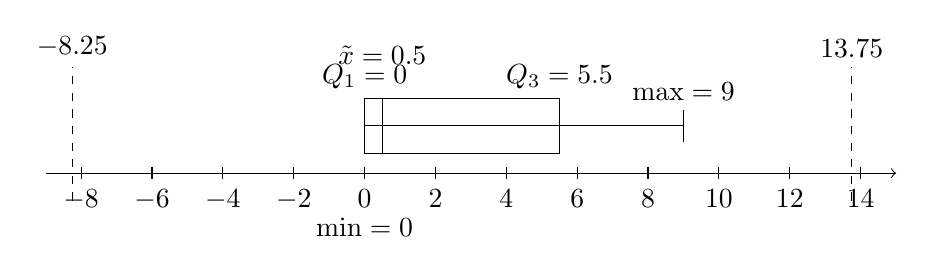
\begin{tikzpicture}[xscale=0.45,yscale=1]
\draw[->] (-9,0) -- (15,0);
\foreach \x in {-8,-6,-4,-2,0,2,4,6,8,10,12,14}
{
    \draw (\x,0.08) -- (\x,-0.08);
    \node[below] at (\x,-0.08) {\(\x\)};
}
\draw[dashed] (-8.25,-0.35) -- (-8.25,1.35);
\node[above] at (-8.25,1.35) {\(-8.25\)};
\draw[dashed] (13.75,-0.35) -- (13.75,1.35);
\node[above] at (13.75,1.35) {\(13.75\)};
\draw (0,0.6) -- (9,0.6);
\draw (0,0.25) rectangle (5.5,0.95);
\draw (0.5,0.25) -- (0.5,0.95);
\draw (0,0.4) -- (0,0.8);
\draw (9,0.4) -- (9,0.8);
\node[above] at (0,0.95) {\(Q_1=0\)};
\node[above] at (0.5,1.25) {\(\tilde{x}=0.5\)};
\node[above] at (5.5,0.95) {\(Q_3=5.5\)};
\node[above] at (9,0.8) {\(\max=9\)};
\node[below] at (0,-0.45) {\(\min=0\)};
\end{tikzpicture}
\end{center}

\newpage

\end{document}
